\documentclass[10pt]{article}
\usepackage{comment}
\usepackage{listings}
\usepackage{graphicx}
\usepackage{psfrag}
\usepackage{amssymb}
\usepackage{amsmath}
\usepackage{algorithm2e}
\usepackage{caption}
\usepackage{epstopdf}
\usepackage{url}
\usepackage{fullpage}


%\usepackage{epsfig}
%\usepackage{subfigure}


\begin{comment}
\newtheorem{theorem}{Theorem}[section]
\newtheorem{proposition}[theorem]{Proposition}
\newtheorem{lemma}[theorem]{Lemma}
\newtheorem{corollary}[theorem]{Corollary}
\newtheorem{definition}[theorem]{Definition}
\end{comment}


\usepackage{enumerate}
\usepackage{float}
\usepackage{flafter}
\usepackage{psfrag}
\usepackage{overpic}
\usepackage{subfigure}
\usepackage{caption}
\usepackage{multirow}
\usepackage{array}

\usepackage{amsmath}

%\usepackage{graphicx}
%\usepackage{caption}
%\DeclareCaptionType{copyrightbox}
%\usepackage{subcaption}
%\usepackage[on]{auto-pst-pdf} % enable psfrag for pdflatex
%\usepackage{xcolor}


\usepackage{epsfig}



\usepackage{color}% Include colors for document elements (required for psfrag)

\newcommand{\psdir}{./sections}
\newcommand{\ldir}{./sections}
\newcommand{\fig}{./sections/fig}
\newcommand{\comm}[1]{}


\def\IL{{\it left}}
\def\IM{{\it middle}}
\def\IR{{\it right}}
\def\IB{{\it bottom}}
\def\IT{{\it top}}


\newcommand{\algref}[1]{Algorithm~\ref{#1}}
\newcommand{\defref}[1]{Definition~\ref{#1}}
\newcommand{\secref}[1]{Section~\ref{#1}}
\newcommand{\figref}[1]{Fig.~\ref{#1}}
\newcommand{\exref}[1]{Ex.~#1}
\newcommand{\tabref}[1]{Table~\ref{#1}}
\newcommand{\thmref}[1]{Theorem~\ref{#1}}
\newcommand{\propref}[1]{Proposition~\ref{#1}}
\newcommand{\efct}[1]{$\langle$ #1 $\rangle$}

\newcommand{\chapref}[1]{Chapter~\ref{#1}}

\newcolumntype{C}[1]{>{\centering\let\newline\\\arraybackslash\hspace{0pt}}m{#1}}


\newcommand{\atlasMgrid}{Atlas MultiGrid}
\newcommand{\cg}{$\cal{G}$}
\newcommand{\cgraph}{active constraint graph}
\newcommand{\sgraph}{stratification graph}
\newcommand{\cs}{$\cal{S}$}
\newcommand{\cd}{colldet}
\newcommand{\pconfig}{parametrized configuration}
\newcommand{\orient}{pose}
\newcommand{\point}{point}
\newcommand{\helix}{molecular composite}
\newcommand{\atom}{atom marker}
\newcommand{\dumbell}{dumbell}
\newcommand{\EASAL}{\texttt{EASAL}}
\newcommand{\Cr}{Cartesian realization}

\newcommand{\tns}{T} %total number of samples
\newcommand{\C}{C} %the collection of interesting atom pairs
\newcommand{\m}{m} %size of S
\newcommand{\stp}{s}


\newcommand{\tol}{$\tau$}
\newcommand{\AC}{A}
\newcommand{\mU}{M}
\newcommand{\aU}{atom marker}
\newcommand{\acg}{G}

\newcommand{\distall}{$C_1$}
\newcommand{\distexist}{$C_2$}

\newcommand{\acgW}{active constraint graph}
\newcommand{\acr}{active constraint region}
\newcommand{\distcons}{Distance Constraints}
%\def\acr{active constraint region}


\newcommand{\cover}{boundaries}


\newcommand{\aview}{atlas view}
\newcommand{\pview}{parametrized chart view}
\newcommand{\rview}{realization view} %configuration space view
\newcommand{\param}{parameter}
\newcommand{\idialog}{intervention dialog}
\newcommand{\ndialog}{node selection dialog}
\newcommand{\atlas}{\textit{atlas}}
\newcommand{\threeRealizable}{$3$-realizable}
\newcommand{\chart}{chart}
\newcommand{\toytwod}{Toy3}
%\newcommand{\toytwod}{Toy$\mathbb{R}^2$}
\newcommand{\toyCayley}{Toy2DCayleyExample}
\newcommand{\toyhelix}{6Atom}
\newcommand{\bighelix}{Toy20}
%\newcommand{\bighelix}{20Atom}
\newcommand{\ctwo}{\ref{eqn:preferredConstraints}}
\newcommand{\cone}{\ref{eqn:constraints}}
\newcommand{\MC}{MC~}
\newcommand{\MD}{MD~}
\newcommand{\custo}{region-specific}
% for lists
\renewcommand{\labelitemi}{$\bullet$}



\def\jorg#1{\textcolor{blue}{#1}}
\definecolor{brown}{RGB}{150,50,50}
\definecolor{pink}{RGB}{219, 48, 122}
\def\old#1{\textcolor{brown}{#1}}
% \def\aysegul#1{\textcolor{red}{#1}}
\def\mred#1{\textcolor{red}{#1}}


% for review
\definecolor{seagreen}{RGB}{48,178,139}
\definecolor{yelloworange}{RGB}{200,146,0}
\definecolor{purple}{RGB}{123,104,238}
%\definecolor{purple}{RGB}{147,112,219}
\definecolor{grayoned}{RGB}{0,0,255}
\definecolor{green2d}{RGB}{0,150,0}
\definecolor{plum}{RGB}{127,0,126}

\newcommand{\aysegul}[1]{{\color{blue}#1}}
\newcommand{\meera}[1]{{\color{magenta}#1}}
\newcommand{\troy}[1]{{\color{seagreen}#1}}
\newcommand{\rahul}[1]{{\color{cyan}#1}}
\newcommand{\joel}[1]{{\color{yelloworange}#1}}
\newcommand{\ruijin}[1]{{\color{plum}#1}}


%opening
\title{EASAL User/Developer Manual}

\author{Aysegul Ozkan, Rahul Prabhu, Ruijin Wu, Troy Baker, \\James Pence, Jorg
Peters, Meera Sitharam \\ University of Florida}

 
\begin{document}

\maketitle
This is a user/developer guide for the EASAL software described in
the accompanying TOMS paper for generating, describing topology and exploring the
assembly configuration space of two rigid sets of points in $R^3$ that are
mutually constrained by distance intervals. Technical concepts and definitions that are 
required to use this software can be found in the main paper.


\section{Introduction}
EASAL generates and describes the key aspects of the topology and geometry of
assembly configuration space of two rigid sets of points in $R^3$
~\cite{Sitharam:2012:EASAL, Ozkan2014MainEasal, Wu2014Virus}. EASAL implements
algorithms that use new theoretical results, some of which are presented in
~\cite{Ozkan2014MainEasal, SiGa:2010, Sitharam:2012:EASAL}.
EASAL is opensource and can be downloaded from
\url{https://www.bitbucket.org/geoplexity/EASAL}. This user guide describes in
depth the key conceptual functionalities, dependencies and installation, and
the major classes and methods in EASAL.  The user can find a detailed example
of how to use the software in the README.md file which can be found along with
the source code. A video presenting the theory, applications, and software
components of EASAL is available at
\url{http://www.cise.ufl.edu/~rprabhu/EASALvideo.mpg}.

\noindent\textbf{Organization:} The remainder of this guide is organized as
follows. Section \ref{functionalities} discusses the main functionalities
offered by EASAL. Section \ref{dependency} gives a description of the software
dependencies and installation instructions. Section \ref{sec:run} describes an
example run to help the user understand how the software is used.
Section \ref{sec:architecture} gives details of the major classes,
attributes and methods to help developers gain an insight into how EASAL  has
been implemented.

\section{Software Functionalities}
\label{functionalities}
This section introduces the main functionalities of EASAL.


\subsection{Input/Output}

\subsubsection{Input}
Input to EASAL is specified using the input window (see \figref{inputwindow}).
The main input features are the following:
\begin{itemize}
		\item \textbf{Two rigid point sets}: \emph{the data for molecule
		(A/B)} field is used to specify the rigid point sets. This accepts the
		data in the pdb format.  The user can either type in the location of
		the input point sets files or select it using the browse option. Once a
		file has been selected, the \emph{set data} option allows the user to edit
		the input data before starting sampling.
\item \textbf{The pairwise distance constraints (potential energy or enthalpy
		function)}: There are three types of constraints.

\item \textbf{Bonding threshold}: This is the range of distances between atoms
		where bond formation is feasible (i.e., the attractive forces dominate). 
		this is given as $\lambda*(r_i+r_j) 
		\pm \delta$ namely the Lennard-Jones well. 
		Here, $\lambda$ is specified by the lambda text field in
		the input window and $\delta$ is specified by the delta text box in the
		input window. $r_i$ and $r_j$ are the radii of the atoms participating
		in the reaction. When predefined interactions are specified, we use those
		for the bond formation and use the bonding threshold only for the hard-sphere
		potentials for the points not involved in the bond formation.

\item \textbf{Collision threshold:} This is the minimum distance between points or atoms. This too is given as $\lambda*(r_i+r_j)
		\pm \delta$.
		
\item \textbf{Predefined Interactions}: Only when the constraints between these pairs are active, are the corresponding configuration space regions explored. 
\end{itemize}

\subsection{Output}
The output is the \emph{atlas} (see \figref{atlas}), i.e., a topologically stratified
set of sample feasible realizations or configurations of the two rigid point
sets. In EASAL the output is visualized by what we call the \emph{sweep view}. One
point set is  held fixed, while the other set is drawn many times to trace out
the set of all feasible realizations.

\begin{figure*}
\begin{center}
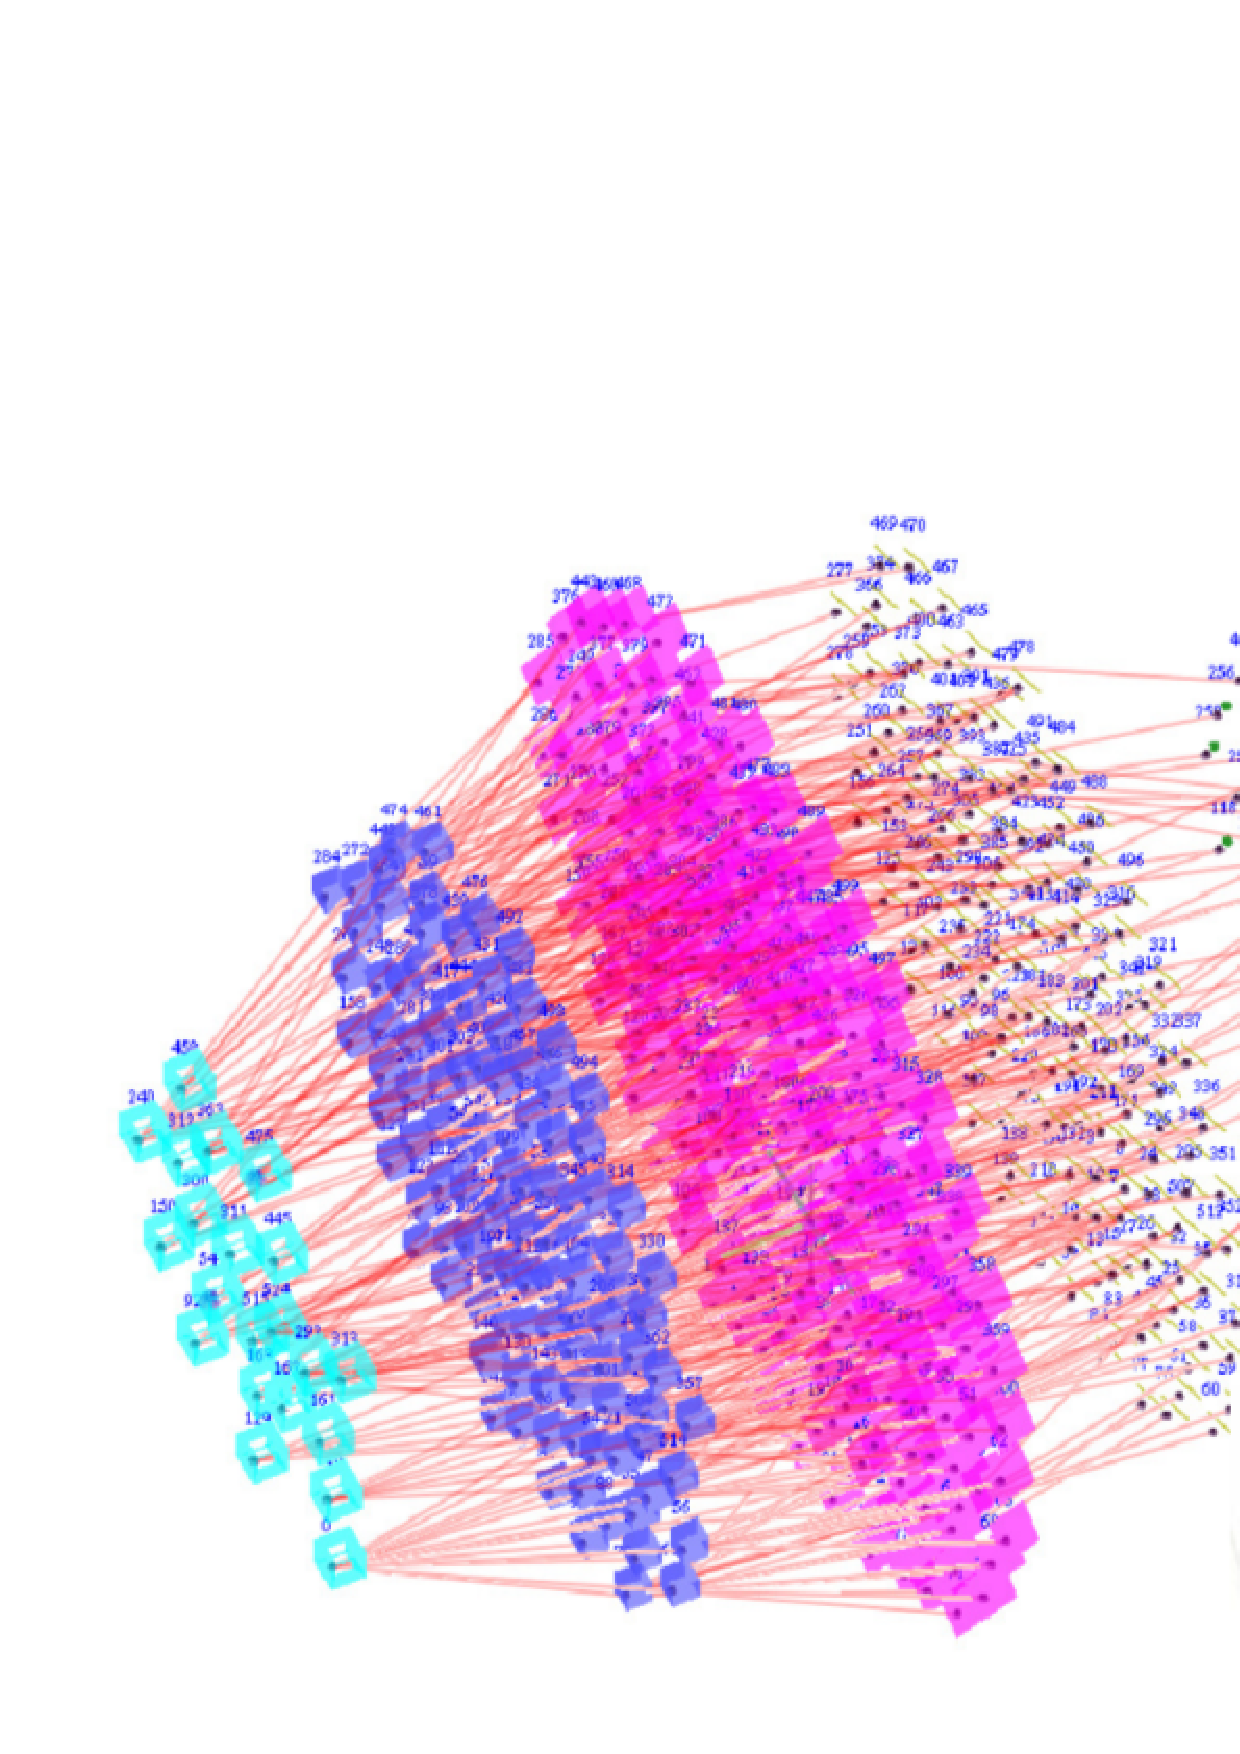
\includegraphics[width=.6\linewidth]{fig/Stratification.png}
\end{center}
\caption{Stratification of an assembly constraint system with atlas nodes of
    dimension 4 (cyan), 3 (blue), 2 (purple), 1 (yellow), and 0 (green). Strata of
	each dimension of the assembly constraint system visualized in the
	lower right inset are shown as nodes of one color and shape in a
	directed acyclic graph. Each node represents an active constraint
region. Edges indicate containment in a parent region one dimension higher.}
\label{atlas}
\end{figure*}


\subsection{Stratification}
When EASAL first starts, the user is presented with the \emph{atlas view} (see
\figref{atlasview}). The atlas view shows the stratification of the
configuration space into regions of various dimensions, known as the active
constraint regions. The stratification is a directed acyclic graph where each
node represents an active constraint region and is associated with an active
constraint graph and edges represent immediate containment of a region within
its parent region.  Here, the user can use the following functionalities. 

\subsubsection{Active Constraint Graph} 
When a node is clicked, EASAL automatically loads the active constraint graph
(see \figref{atlasview}) associated with that node in the bottom left corner.
This active constraint graph shows only the participating points from each set.
A solid edge between two points indicates a constraint and a dashed edge
indicates a parameter between two points belonging to different sets. It has to
be noted that the points in the same set already form a clique (not shown in
the graph).

\subsubsection{Finding Bounding Regions} 
Clicking \emph{tree} (see \figref{atlasview}) after selecting a particular node from
the atlas shows us all the bounding regions of that node. In terms of the atlas, it shows  
the ancestors and descendants of that node . Since an edge in the graph represents 
containment, this feature allows us to inspect the containment of regions.
Note that the bounding regions are also shown in the Cayley space view.

\subsubsection{Finding Paths Between Nodes with 6 Active constraints}
The atlas output by EASAL can be used to generate all the paths between any two active
constraint regions along with their energies. Once the atlas has been generated, 
finding paths is \emph{nearly instantaneous}. The path topology of 
the assembly configuration space is crucial for understanding assembly kinetics.

Of particular interest is finding paths between two lowest energy
configurations with 6 active constraints or 0D nodes of the atlas with effectively rigid 
configurations. We are mainly interested in paths through active constraint regions with 5 
or 6 active constraints (which are one step higher energy and have one fewer constraint). 
Such paths represent a continuous one degree of freedom motion.

Whenever the user clicks on two nodes in succession, EASAL finds the path between the two 
nodes, if it exists, and writes this path as a series of nodes to the 
``paths.txt'' file. Once the sampling has been completed, EASAL computes the total number of paths of a particular length between every pair of vertices and writes the entire matrix to the ``path\_matrix.txt'' file. The user can specify lengths by setting the ``path\_length'' parameter in the settings.ini file.

\subsubsection{Sampling Options} 
The user can at any point stop the current sampling mode and redirect the
sampling. The various options available are:
\begin{itemize}
\item \textbf{Stop Sampling}: Clicking this button stops the sampling of the
		atlas and presents options to redirect the sampling.
\item \textbf{The Constraint Selection Dialogue Box}: This dialogue box (see Figure~\ref
		{CSD}) allows the user to select a particular node from the atlas and start
		sampling from that node. This feature gives users the flexibility to
		explore regions of the graph that are more relevant to them. The user
		can select a node by either specifying a node number or by specifying
		active constraints between the point sets. The spheres with the indices
		denote the atoms. A thick line between the atoms indicates a
		participating bond.  Here, the first constraint is mandatory and hence
		does not have a \emph{connect} check box next to it. The rest of the Active
		constraints are optional and the user may choose up to six.
		\begin{figure}[h] 
				\centering 
				\includegraphics[scale=0.5]{fig/DumbbellSelection.png} 
				\caption{Constraint Selection Dialogue} 
				\label{CSD} 
		\end{figure}

\item \textbf{CUR}: On clicking this, the sampling starts from the node that is
		currently selected and ends when the tree in which the node is present
		is fully sampled.
\item \textbf{Cleanup}: Clicking this completes sampling on all partially
		sampled trees.
\item \textbf{A-S}: A-S stands for Auto-Solve. This button starts sampling in
		the auto-solve mode. This is the default sampling mode. When starting
		afresh in this mode, EASAL generates all possible 4D and 5D root nodes
		depending on the user input. Then it proceeds to recursively sample all
		these nodes till the atlas generation is complete. If there is a
		partially generated atlas, this mode of sampling completes	 the
		unfinished trees and then proceeds to sample all the other root nodes.
\item \textbf{BFS}: Clicking this button forces EASAL to explore the atlas in
		a breadth first fashion which it otherwise does in a depth first
		fashion. In this mode of sampling, EASAL starts from the
		node currently selected and samples its subtree to completion.

\end{itemize}

\subsubsection{Dimension of the root node}
By default, the dimension of the root node of the atlas is 5, which means that
the root node has one bond and 5 parameters. The \emph{4D root node} option in the
\emph{advanced options} (see \figref{advancedoptions}) allows the user to change
this and make the root node a 4D node. With a 4D root node, there are 2 bonds
and 4 parameters in the root node.

\subsection{Convex Cayley Parametrization}
After selecting a node, the user can view its Cayley configuration space shown
in the \emph{Cayley space view} (see \figref{Cayleyspaceview}). The Cayley space
view shows the active constraint region in the Cayley parametrized chart
representation for a particular node.

\subsubsection{Inspect Cayley Points}
The user can view the Cayley points in the Cayley Space View (see
\figref{Cayleyspaceview}). The Cayley points are shown on a 3D grid. For nodes
of dimension higher than 3d, one slider per extra dimension is given to view
the points in the $4^{th}$ and $5^{th}$ dimensions.

\noindent\textbf{Categorization of Cayley points:} In the Cayley Space View
(see \figref{Cayleyspaceview}), initially green points are shown which
correspond to all the realizable points in the Cayley space. Clicking on the
red square at the bottom shows the points that have collision.  Clicking
the red square also shows two more options viz., cyan and pink. The cyan points
represent the points which have angle violations and the pink points represent
points which have distance violations. Clicking on the blue square shows all the
points sampled. The blue points represent geometrically infeasible points.

\subsubsection{View Boundaries}
EASAL allows the user to inspect the points that form the boundary between a
region and its parent/child. The boundaries option allows the user to inspect
the boundaries of the Cayley space. The user can step through each of the
boundaries using arrows provided.

\subsubsection{Step Size}
EASAL uses Cayley grid sampling to sample the Cayley space. The user can
specify this step size in the input window (see \figref{inputwindow}). Another
option available to the user is to choose the \emph{dynamic step size} option in the
advanced window (see \figref{advancedoptions}). This tells EASAL to determine 
the step size based on the volume of the space it is sampling. Once a space has
been sampled, there is always the option of refining the sampling. This can be
done by selecting the \emph{refine sampling} option in the atlas view whereupon
EASAL halves the step size and re-samples all the sampled spaces.

\subsection{Cartesian Realization}
The realization view (see \figref{realizationview}) in EASAL shows the
Cartesian realization of the Cayley points. 

\subsubsection{View the sweep and flips of the Cartesian realization}
The sweep feature of a realization keeps one of the point sets units fixed and
draws all the possible orientations the other point set can take relative to the
first one (see \figref{realizationview}). The user can view the sweep. 
When the sweep is being displayed, the user can use
the arrow keys to view the different flips.


\subsubsection{View realization along boundaries}
Clicking on the \emph{boundaries} control allows the user to view the realizations
along the boundary region. The user can view it walk through the boundary
realizations using the arrows provided. Different colors are used to indicate
the realizations along different boundaries.

\subsubsection{View all realizations}
The user can use the video controls at the bottom (see
\figref{realizationview}) to display all the realizations of a region one after
the other. This differs from the sweep view in that sweep view shows all the
realizations at the same time.


\section{Dependencies and installation}
\label{dependency}
This section discusses all the dependencies EASAL requires to run.

\begin{itemize} 
  \item Though technically, this should work on any UNIX variant platform with little to no modifications, it has been thoroughly tested to work on the following platforms. 
  \begin{itemize}
	\item Ubuntu 12.04 or higher.
	\item Fedora 22 or higher.
	\item OS X 10.8 Mountain Lion.
\end{itemize}
  \item We use Version 2.0 of the Eigen library for linear algebra
		  computations. All necessary files pertaining to Eigen required by
		  EASAL are provided with the source code in the \emph{include}
		  directory.  
   
   \item For the GUI, we use OpenGL for visualization and the
		  opensource fox-toolkit Version 1.6 for windowing. See the
		  installation section for instructions on installing the necessary
		  libraries.  
		  
   \item We use simpleini to read the settings from the
		  settings.ini file. All necessary files pertaining to simpleini are
		  provided with the source code in the include directory.
   
   \item EASAL has been tested on the NVIDIA graphics card with the NVIDIA
		  proprietary driver (Version 331 or higher).  \item EASAL is written
		  in C++ and hence requires G++ Version 4.8 or higher or Clang Version 3.8 or 
		  higher to compile the source code. 
		  
  \item EASAL uses the GNU Make utility to compile the source files. Make
		  Version 4.1 is required.
\end{itemize}

 
\subsection{Installation}
The software can be run either as a terminal application or with its associated GUI.
The steps for running each of these versions has been explained here. You will need to download and install some third party libraries and update the makefile provided before you can successfully compile and run EASAL in the GUI mode.  
\begin{itemize}
	\item Install GLUT 
	  \begin{itemize}
	  \item On Ubuntu 
	  	  \begin{itemize}
	  	  	\item sudo apt-get install freeglut3 freeglut3-dev binutils-gold
		  \end{itemize}
	 \item On Fedora
	 \begin{itemize}
	  	  \item sudo yum install freeglut-devel mesa-dri-drivers mesa-libGL 
\end{itemize}
	  \end{itemize}
     \item Install FOX-Toolkit (Version 1.6)
	   \begin{itemize}
		   \item Download the fox library headers from \url{http://fox-toolkit.org/} and extract it.
		   \item On Ubuntu
		   \begin{itemize}
	   	   		\item sudo apt-get install libfox-1.6-0 libfox-1.6-dev
			\end{itemize}
		   \item On Fedora
		   	\begin{itemize}
		   		\item Download fox toolkit from \url{http://fox-toolkit.org/}
				\item Extract it using ``tar -xvzf libFox-1.6.X.tar.gz''
				\item Run configure using ``su ./configure''
				\item Install using ``su make install''
			\end{itemize}

	   \end{itemize}
	 \item Install GNU Make
	   \begin{itemize}
	   	   \item On Ubuntu 
	   	   \begin{itemize}
			\item sudo apt-get install make
		   \end{itemize}	
		   \item On Fedora
		   \begin{itemize}
			\item yum install make
\end{itemize}
		   \end{itemize}
	 \item Edit the Makefile to point to your versions of FOX.
	   \begin{itemize}
	   	   \item Edit the line 
	   	   	 ``include\_dirs = -I /usr/lib/fox-1.6.50/include/ -I ./include/''\\
	   	   	 and replace \\
	   	   	 /usr/lib/fox-1.6.50 with the location you have downloaded and extracted the fox headers.
		\end{itemize}
	 \item Run \emph{make} from the root/build directory.
	 \item To run EASAL run \emph{``bin/EASAL''} in a terminal from the root/build directory.
\end{itemize}% subsubsection  (end)




\section{Sample Run}
\label{sec:run}
This section shows a sample run of EASAL in both the Terminal mode and the GUI mode.

\subsection{Terminal Mode}
\label{sub:TMode}
When the software is run in the terminal mode, all input is specified using the settings.ini file. 

% subsection  (end)
\subsection{GUI mode}
\label{sub:GUIMode}

% subsection  (end)

\begin{itemize}

\item Run EASAL from the command line by running the following command.
    \emph{\$bin/EASAL}

\begin{figure}[h]
	\centering
	\includegraphics[scale=0.5] {fig/InputWindow.png}
	\caption{- In the input window, select the following either using the
			browse option or by entering the text in the text box provided\\
    - Data for Molecule A - files/A.pdb\\
    - Data for Molecule B - files/B.pdb\\
    - Distance Data - files/source\_files/union\ computed\ desired\ distances.txt\\
    - Data Directory - data/\\
    - Enter the values for Bonding Thresholds and step size .
}
	\label{inputwindow}
\end{figure}


\item The user can then click on the \emph{advanced options} button to set advanced
		user inputs. This opens a new pop-up where the user can enter either
		enter the data or choose to accept the default values.

\begin{figure}[h]
\centering
\includegraphics[scale=0.5] {fig/AdvancedOptions.png}
\caption{Advanced Options Window}
\label{advancedoptions}
\end{figure}

\item Click on \emph{accept}. This opens the Atlas View.

\begin{figure}[h]
	\centering
	\includegraphics[scale=0.5] {fig/AtlasView.png}
	\caption{The Atlas View in EASAL . (A) Button to stop the sampling. (B) Button
to start the constraint selection dialogue box. (C) Button to continue sampling
the current tree. (D) Button to Clean Up Sampling. (E) Button to run EASAL in
the Auto-Solve mode. (F) Button to start exploring the Atlas in a breadth first
fashion. (G) Button to refine the sampling using a smaller step size. (H)
Active Constraint graph of the node selected. The spheres with the indices
denote the atoms. A thick line between the atoms indicates a bond and a dotted
line indicates a parameter. (I) Button to toggle Tree View. (J) Button to
toggle Gravity. (K) Cartesian realization of the current node.}
\label{atlasview}
\end{figure}

\item In the Atlas View, we initially see a root node at the center of a 3D
		grid. As and when more nodes are discovered, they are populated on the
		Atlas.

\item When the tree view is on, it shows only the ancestors and descendants of
		the node selected. When it is off, it shows the entire atlas. This can
		also be achieved by clicking the Tree control at the bottom.

\item In this view, the user can control how the sampling proceeds by using any
		of the controls on the left side of the atlas. The different controls
		available are (in the order they appear)
    - Stop Sampling.
    - Constraint Selection Dialogue Box.
    - Sample the Current Tree.
	- Sample all Incomplete Trees.
	- Auto-Solve.
    - BFS Sampling.
    - Refine Sampling.

\item Clicking on a particular node does the following - Loads the Active
		Constraint Graph at the bottom left corner.  - Loads the Cartesian
		realization for that node in the top right corner if the sampling for
		the node is complete.

\begin{figure}[h]
	\centering
	\includegraphics[scale=0.5] {fig/CayleySpaceView.jpg}
	\caption{Cayley Space View. The points outside the box show the boundary
points. The points in the box show the various Cayley points. From left to
right Good points, Collision points, points which violate the steric
constraints and all the points sampled.}
\label{Cayleyspaceview}
\end{figure}


\item Pressing the space bar after selecting a node takes the user to the
		Cayley space view of that node.

\item In the Cayley Space View, initially green points are shown which
		correspond to all the realizable points in the Cayley space.

\item Clicking on the Red square at the bottom, shows the points that have
		collision. Clicking the red also shows two more options viz, cyan and
		pink. The Cyan points represent the points which have angle collision
		and the pink points represent points which have distance collision.

\item Clicking on the Blue square shows all the points sampled including, the
		good, the collision and the unrealizable.

\item Clicking on the Boundaries shows the boundary points and the user can
		step through them along each dimension.

\begin{figure}[h]
	\centering
	\includegraphics[scale=0.5] {fig/RealizationView.png}
	\caption{Realization View. The images in the box show the different
		realizations along different boundaries.}
		\label{realizationview}
\end{figure}

\item Pressing the space bar here takes the user to the \emph{realization view}.

\item Pressing \emph{v} on the keyboard generates the sweep view of the point set.

\item Once the sweep view is generated, the user can use the up and down arrow
		keys to view all the flips of the point set.

\item Clicking on boundaries shows the different realization along different
		boundaries.

\item Clicking on the video controls at the bottom and clicking the play button
		on it animates and shows all the possible realizations of the point set.
\end{itemize}


\subsection{Major Classes and Architecture of \texttt{EASAL}}
\label{sec:classes}

The core classes are AtlasBuilder, ActiveConstraintGraph, CayleyParameterization, ConvexChart, and CartesianRealizer.

\troy{Should the fundamental classes (such as MolecularUnit, Orientation, Atom, etc.\ be discussed? Or at least mentioned briefly as being basic and easy to understand.)}


\begin{enumerate}

%---------------------------------------------------------------------------------------------------------------
\item \textsf{Atlas} class: the directed acyclic graph that represent the relation of active constraint regions

\smallskip
Major Attributes:

\noindent --  \textsf{atlas}: set of AtlasNodes

\noindent --  \textsf{atlasRoot}: set of AtlasNodes that take place at the root of atlas.

\smallskip
Major Methods:\\
\smallskip
\noindent --  \textsf{search(node)}: depth first search the atlas from one of the node's ancestor to check whether the node exists in atlas or not. \\
It is used to avoid repeated sampling of the same region.
%During sampling when the boundary of the region is reached, it is necessary to check whether the boundary child region has been sampled before or not.
The time complexity of the search is $O(log(\text{depth of the tree})) = O( log(6) )$ considering we stop creating child nodes with overconstrained ActiveConstraintGraphs.\\


%---------------------------------------------------------------------------------------------------------------
\item \textsf{AtlasNode} class: node in the Atlas, each represents an active constraint region labeled by ActiveConstraintGraph.

\smallskip
Major Attributes:

\noindent --  \textsf{acg}: the active constraint graph of the node.\\
\noindent --  \textsf{region}: the set of Cayley points in the active region.\\
\noindent --  \textsf{connection}: the id of the child nodes in the atlas that represent the boundary of this node's region.\\



%---------------------------------------------------------------------------------------------------------------
\item \textsf{ActiveConstraintGraph} class: is used to store the set of active constraints and the corresponding vertices.

\smallskip
Major Attributes:

\noindent --  \textsf{activeConstraints}: set of \atom\ index pairs that represent contacts

\noindent --  \textsf{verticesA}: participating \atom\ indices from first \helix

\noindent --  \textsf{verticesB}: participating \atom\ indices from second \helix

\noindent --  \textsf{parameters}: set of \atom\ index pairs that represent parameters

\smallskip
Major Methods:\\
\smallskip
\noindent --  \textsf{completeTo3by3Graph()}: add \atom\ to make sure there are at least 3 \atom s from each \helix\ so that the graph is realizable.
While choosing additional atoms, it has 2 options, choosing the closest atom to each other or the atoms that leads certain angle. \\
\smallskip
\noindent --  \textsf{parameterMinDeviation()}: An alternative method to pick the parameters for $5$ dimensional region such that the range of each parameter has similar length.
It aims sampling more uniformly on Cartesian space by setting Cayley parameter space as spheric as possible.
%It is designed for dimension $5$, i.e., for ActiveConstraintGraph with only one active constraint. It adds extra 2 \atom s from each \helix\ and sets parameters that will yield spheric \chart. i.e. the range of each parameter has similar length. \\


%---------------------------------------------------------------------------------------------------------------
\item \textsf{ActiveConstraintRegion} class: the set of feasible Cayley Points generated by sampling

\smallskip
Major Attributes:

\noindent --  \textsf{space}: set of feasible Cayley Points

\noindent --  \textsf{witspace}: set of feasible witness Cayley Points achieved from ancestor

\smallskip
Major Methods:\\
\smallskip
\noindent --  \textsf{convertSpace(activeConstraintRegion)}: Re-parametrize another region using this region’s parameters.
%One orientation can be represented by different Cayley points according to different parametrization.
%This method converts each Cayley point of input activeConstraintRegion to the Cayley point parametrized by this region's parametrization. \\

%---------------------------------------------------------------------------------------------------------------
\item \textsf{CayleyPoint} class: a multi-dimension point in the Cayley parameter space, and the corresponding Cartesian space orientations of the \helix.

\smallskip
Major Attributes:

\noindent --  \textsf{data}: value of the Cayley parameters (non-edge length)\\
\noindent --  \textsf{orients}: set of Cartesian space Orientations of the \helix\ that, computed by realizing the active constraint graph with given length of edge/non-edges.\\

%We note that we use \emph{configuration} throughout to refer to
%a choice of Cayley parameters, typically distances between molecules,
%while the actual placement of the molcules with respect to one another
%in Cartesian $xyz$-space is called a \emph{realization}.
%---------------------------------------------------------------------------------------------------------------
\item \textsf{Orientation} class: the Euclidean transformation of \helix.
%Orientation stores only the necessary information to compute transformation matrix that will yield to Cartesian realization for the entire \helix\.

\smallskip
Major Attributes:

\noindent --  \textsf{FromB}: Cartesian coordinate of three \atom s from the \helix\ before the transformation.\\
\noindent --  \textsf{ToB}: Cartesian coordinate of three \atom s from the \helix\ after the transformation.\\
\noindent --  \textsf{connections}: the set of node indices that this orientation belongs. An orientation can take place in the boundary of multiple regions.\\

%---------------------------------------------------------------------------------------------------------------
\item \textsf{CayleyParameterization} class: choose non-edges in an ActiveConstraintGraph that complete the graph into 3-tree. Those non-edges are called the parameters.
The complexity of the sampling algorithm varies based on the choice of non-edges and the order in which they are fixed.
%should we move ordering parameters and related routines such as createTetrahedras, boundaryComputationWay and updateList to the convexchart class???

\smallskip
Major Attributes:

\noindent --  \textsf{partial3tree}: a flag to show whether ActiveConstraintGraph is partial 3-tree or not.

\noindent --  \textsf{parameters}: set of \atom\ pairs that represent non-edges

\noindent --  \textsf{tetra}: the ordered tetrahedra set that helps to define the order of parameters that will be important later during sampling procedure.
This data is later on passed to ConvexChart and CartesianRealizer to help their computations.

\noindent --  \textsf{updateList}: adjacency map for dependency of parameters. It provides the set of parameters whose range will be updated when one parameter fixed.

\noindent --  \textsf{boundaryComputationWay}:  inequalities that express the range of a parameter can be classified into either a linear or non-linear class.
This variable is characterization of the parameter that tells what inequality is needed to compute parameter range, i.e., triangular or tetrahedral inequality.

\smallskip
Major Methods:\\
\smallskip
\noindent --  \textsf{defineParameters()}:
The parameters $H$ of an active constraint graph are selected as maximal 3-realizable (3-tree) extension by leveraging the convex parametrization theory. % \cite{paper}.
It sets parameters retaining parent node's parameters as much as possible. So that we do not need to do much change on the parameter list as we dive into child regions.
For this purpose a look up table is created, that gives the parameters for a given constraints.\\
\smallskip
\noindent --  \textsf{createTetrahedras()}:
finds a 4 clique as a base tetrahedra. Then complete 3-tree is built up from a base tethedra by adding, at each step, a new vertex
edge-connected to the face of a tetrahedra. Store the tetrahedras in the order they are created in attribute \textsf{tetra}.\\
\smallskip
\noindent --  \textsf{orderParams()}: order of non-edges can guarantee efficient
sampling where finding bounds for each non-edge is either solving a linear inequality or
solving a single quadratic of one variable. \cite{ugandhar}
%the ordering of parameters is important to have exact convex chart while sampling. There is existing theories to solve it. However it was slow, so we have used our own heuristic way.

Here we use a simplified routine to order parameters with the following heuristics:\\
Fixing a non-edge, requires the range computation for the non-fixed parameter that takes place in same tetrahedra.
Lets D be a graph with vertices as parameters and edges representing if the two parameters takes place in the same tetrahedra.
Then which parameter should we choose as a root so that the depth of the graph D is minimum.
Here we aim the cascade of range computations to minimize.

In order to achieve this goal:\\
Order the parameters in the same order you built the tetrahedras. If there is one parameter in a tetrahedra, it is trivial, just add it to paramter list. Otherwise, prioritize the parameter which is shared by more tetrahedras, i.e., the vertex with max degrees.\\

%optimization


%---------------------------------------------------------------------------------------------------------------
\item \textsf{ConvexChart} class: is used to determine the \chart\ that parameterize the regions, i.e., it computes the range of parameters of ActiveConstraintGraph. \\
An exact convex chart yields feasible Cayley points for the current active constraint region.
The resulting Cayley configuration space is convex, before collisions or other (e.g.\ angle) constraints are introduced.
The range of parameters are computed by triangle and tetrahedra inequalities.

\smallskip
Major Attributes:

%\noindent --  \textsf{connections: fixed distance values of ActiveConstraintGraph such as active constraints or edges being taking place in one helix.
\noindent --  \textsf{maxconnections}: upper bound of the parameters' range

\noindent --  \textsf{minconnections}: lower bound of the parameters' range

\noindent --  \textsf{paramconnections}: current value of parameters

\smallskip
Major Methods:\\
\smallskip
\noindent --  \textsf{initializeChart()}: it initalizes the boundaries of convex chart.
Tighter bounds are given in \cite{ugandhar}.\\

\smallskip
\noindent --  \textsf{computeRange(v1, v2)}: computes the range of the parameter v1-v2 in order to eliminate sampling infeasible grid points.\\
Range computation is required in every iteration for dependent parameters.
When there is one parameter in a tetrahedra, the range of parameter can be computed through tetrahedral inequalities.
If there are 2 unfixed parameters at the moment in a tetrahedra, then the range of one of the parameters will be computed through triangular inequalities and fixed. And the range of other parameter will be computed through tetrahedral inequalities. The range computation way depends on the order of parameters. \\
\smallskip
\noindent --  \textsf{setMinMaxByTriangleInequalityParam(v1, v2)}: computes the range of the non-edge v1-v2 through triangular inequalities. uses all triangles that this edge is shared.\\
\smallskip
\noindent --  \textsf{setMinMaxByTetraHedraInequality(v1, v2, tetraHedra)}: computes the range of the non-edge v1-v2 through tetrahedral inequality using input tetrahedra\\
\smallskip
\noindent --  \textsf{stepGrid}: sets parameter point to the next grid point within the computed range.\\
%Range computation is required in every iteration for dependent parameters.
%Triangular inequality and tetrahedral equality is used to find boundary hence eliminate sampling infeasible grid points.\\

%stepGrid: after stepping on pth parameter, it should update min max range for params from 0th till p'th  not just p'th parameter because if p'th parameters value is changed then that means every previous parameters feasible range will change.
\smallskip
\noindent --  \textsf{stepNeighbour()}: sets parameter point to the neighbour grid point in all dimensions consecutively.\\
\smallskip
\noindent --  \textsf{stepGridBinary()}: sets parameter point to the somewhere between current point and neighbour grid point according to binary search procedure in boundaryDetection.\\


%---------------------------------------------------------------------------------------------------------------
\item \textsf{CartesianRealizer} class: %(?naming CartesianOrientatior)
contains routines that computes Orientation that represents transformations of the rigid \helix\ s relative to each other.
It computes Cartesian realization of an ACG with the parameter lengths taken from cayleyPoint and active constraint lengths for a specific flip.
It intentionally ignores the remainder of the assembly constraint system, namely atom markers not in G and their constraints.

\smallskip
Major Attributes:

\noindent --  \textsf{positions}: Cartesian coordinates of vertices in ActiveConstraintGraph

\noindent --  \textsf{pconnections}: contains all fixed distances plus current distance values of non-edges of ActiveConstraintGraph

\smallskip
Major Methods:\\
\smallskip
%actually no need for whole convexChart, what you need is cayleyPoint to achieve current paramValues, and fixed distances of inter/intra molecule
\noindent --  \textsf{computeRealization(activeConstraintGraph, convexChart, flipno)}: computes the Orientation by leveraging partial 3-tree techniques.
activeConstraintGraph which is a complete 3-tree is built up from a base tethedra by adding, at each step, a new vertex
edge-connected to the face of a tetrahedra.\\
\smallskip
\noindent --  \textsf{setmybase(tetrahedra)}:  finds Cartesian coordinates of the vertices of tetrahedra by known edge lengths \\
\smallskip
\noindent --  \textsf{findLocation(vertex, face)}: finds Cartesian coordinates of the vertex that is connected to the face of a tetrahedra\\
%\noindent --  \textsf{findLengthsAcordingToTwoKnownPoints(vertex): sets the distance of any undefined edge connected to vertex. (actually you may put this in the above method, if not worth to talk)

%---------------------------------------------------------------------------------------------------------------
\item \textsf{ConstraintCheck} class: is designed to check whether any non-active constraints become active or whether they are violated.

User have the option to define set of constraints of interest. In that case, new constraint activation check will be done only for this set.
For an input Orientation, ConstraintCheck first computes the Cartesian realization for the entire \helix\ then passes it to the subroutines to do user specified constraint check such as steric constraints, tethering constraints or angle constraints.\\


%---------------------------------------------------------------------------------------------------------------
\item \textsf{AtlasBuilder} class: populates the ActiveConstraintRegion for each activeConstraintGraph by sampling inside the boundaries of its ConvexChart.
It creates and explores only regions that contain at least one Cartesian realization, witness point.
If activeConstraintGraph is not partial 3-tree, then the region is populated by ray tracing, i.e., witness points coming from all ancestors.


\begin{comment}
AtlasBuilder currently follows predefined direction to walk through on sampling space.
It can be modified to have a recursive sampling so that wastefully sampling the body of the violated region will be  eliminated.
Since recursive sampling can identify the boundary of the violated region by sampling from all directions.
%
Also again recursive sampling can identify the boundary of feasible region hence would eliminate boundary computation in every step. :)
(Actually even in predefined direction sampling, you do not need to compute boundaries, just keep sampling, if you hit a neg volume then stop sampling in that direction.! )
(No, you may jump to an infeasible region and stuck there, it should always start sampling withing feasible region computed by chart.)
\end{comment}

\smallskip
Major Attributes:

\noindent --  \textsf{positions}: Cartesian coordinates of vertices in ActiveConstraintGraph

\smallskip
Major Methods:\\
\smallskip
\noindent --  \textsf{startAtlas()}: for each (bi)tether creates root atlasNode labeled with a contact graph $G_F$ where $F$ is the (bi)Tether, i.e., $1$ (or $2$) specific contacts. Then calls sampleExplore for that atlasNode.\\
\smallskip
\noindent --  \textsf{sampleExplore(atlasNode)}: elaborated in Section \ref{sec:sampleExplore}.\\
\smallskip
\noindent --  \textsf{determineStepSizeDynamically()}: finds out \stp\ by given \tns, total number of samples. Each 5d-atlas node has its own \stp\ computed by volume of Cayley parameter space of the node over total number of samples per node. The number of samples per node roughly can be computed by \tns\ over total number of root(starter) atlas nodes, \m. The number of samples in child nodes are ignorable since the volume of regions in low dimensional nodes are ignorable compared to the regions of high dimensional nodes. \\
%To be more specific, the number of samples distribution over nodes would be proportional with the sum of radius of the tether of the node.
%need explanation how the cayley volume is computed, i just stepped on ot without realizing within the chart. since no realization it is fast. but since chart boundary is computed in most of the steps, kind of slow.
\smallskip
\noindent --  \textsf{boundaryDetection()}: elaborated in Section \ref{sec:boundaryDetection}.\\
\smallskip
\noindent --  \textsf{rayTracing()}:
a recursive routine to explore regions that do not have an active constraint graph that is a partial 3-tree, by inheriting samples from
the parent node(s).\\


%---------------------------------------------------------------------------------------------------------------
\end{enumerate}






\bibliographystyle{plain}
\bibliography{easal}

\end{document}
